\providecommand{\main}{../../..}
\documentclass[\main/main.tex]{subfiles}
\begin{document}

\subsection{Exercise 12}
The following problem is given:

\begin{align*}
  \min f_1\rnd{x} = x_1^2 + 4x_2^2 -2x_1 -16x_2 \\
  \min f_2(x) = -5x_1 -x_2                      \\
  x_1^2 + x_2^2 & \leq 8                        \\
  x_2           & \geq 0                        \\
\end{align*}


Represent the utopy point $U$ in the space of the objectives.

\subsection{Exercise 12 resolution}
The domain is an semicircle with a radius of $\sqrt{8} = 2\sqrt{2}$, the section in the positive ordinates.

\begin{figure}
  \begin{subfigure}{0.49\textwidth}
    \xygraph{-2.8284}{2.8284}{0}{2.8284}{-20}{
      x^2 + y^2 <= 8
    }{x^2 + 4*y^2 - 2*x - 16*y}
    \caption{The objective function $f_1$}
  \end{subfigure}
  \begin{subfigure}{0.49\textwidth}
    \xygraph{-2.8284}{2.8284}{0}{2.8284}{-20}{
      x^2 + y^2 <= 8
    }{-5*x-y}
    \caption{The objective function $f_2$}
  \end{subfigure}
\end{figure}

The minima of the first objective function is identified geometrically, as the center of $\bmx = (1,2)$, with a value of $f_1 = -17$.

The minima of the second objective function is identified via the maximum growth coefficient $\frac{1}{5}$:

\[
  \begin{cases}
    x_1^2+x_2^2 = 8 \\
    x_2 = \frac{x_1}{5}
  \end{cases}
  \Rightarrow
  \begin{cases}
    x_1^2+\frac{x^2_1}{25} = 8 \\
    x_2 = \frac{x_1}{5}
  \end{cases}
  \Rightarrow
  \begin{cases}
    \frac{26x^2_1}{25} = 8 \\
    x_2 = \frac{x_1}{5}
  \end{cases}
  \Rightarrow
  \begin{cases}
    x^2_1 = \frac{100}{\sqrt{13}} \\
    x_2 = \frac{x_1}{5}
  \end{cases}
  \Rightarrow
  \begin{cases}
    x_1 = \frac{10}{\sqrt{13}} \\
    x_2 = \frac{2}{\sqrt{13}}
  \end{cases}
\]

The minima is $f_2^{*} = -\frac{52}{\sqrt{13}}$

\begin{figure}
  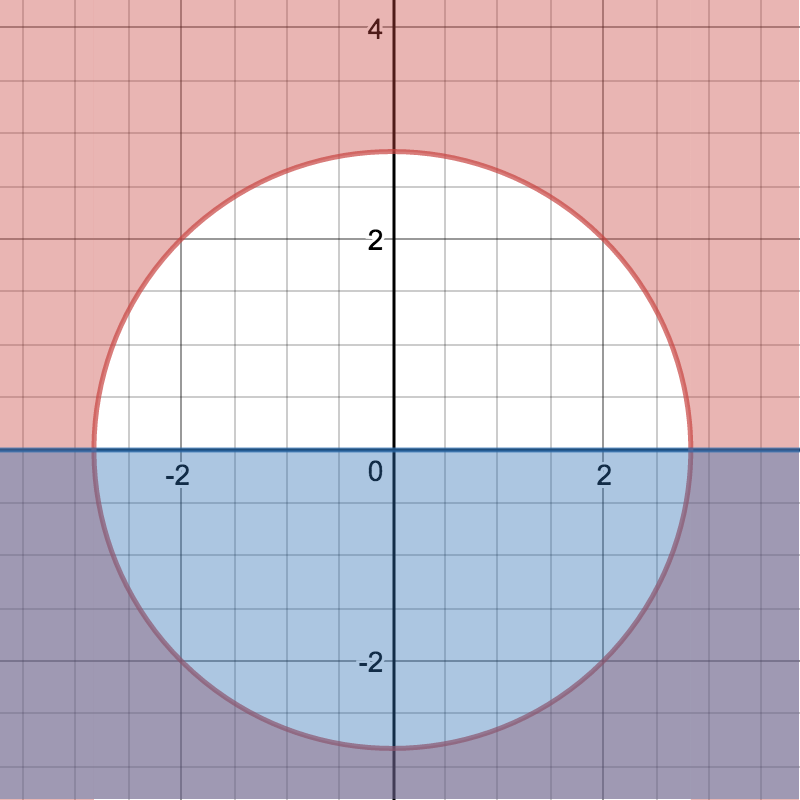
\includegraphics[width=0.4\textwidth]{es12-maut}
\end{figure}

\end{document}